\documentclass[12pt]{article}

\usepackage{sbc-template}

\usepackage{graphicx,url}

\usepackage[brazil]{babel}   
\usepackage[utf8]{inputenc}  

     
\sloppy

\title{Proposta de 1º Trabalho prático - Desenvolvimento em Linux}

\author{Bruno Tomé\inst{1}}

\address{Instituto Federal de Minas Gerais - Campus Formiga (IFMG)\\
  CEP 35570-000 -- Formiga -- MG -- Brasil
  \email{ibrunotome@gmail.com}
}

\begin{document} 

\maketitle
     
\begin{resumo} 
	Este trabalho consiste em desenvolver scripts em sed, awk e bash para resolver algum problema prático selecionado pelo aluno.
\end{resumo}


\section{Descrição do problema}
	
	O problema consiste em realizar o download das imagens de um perfil público na rede social Instagram e organizá-las em pastas de acordo com o nome de usuário e resolução das imagens obtidas.
	
\begin{figure}[ht]
\centering
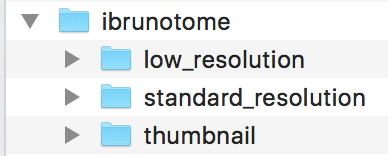
\includegraphics[width=.5\textwidth]{fig1}
\caption{Exemplo de estrutura de organização das imagens}
\end{figure}

\section{Motivação e relevância}
	
	Trabalho há alguns anos com publicidade em redes sociais e gostaria de checar se é possível e viável trabalhar com APIs no terminal do Linux, em JSON (utilizado pela maioria das APIs).
	
	Com o script proposto será possível armazenar localmente todas as fotos do usuário na rede social, uma espécie de backup do conteúdo postado na rede.
	
\section{Resumo da solução proposta (etapas)}

	A primeira etapa é tratar o usuário digitado com o comando sed, por exemplo, um usuário de Instagram válido é ibrunotome, e não @ibrunotome ou https://www.instagram.com/ibrunotome, logo com o comando sed será possível apagar as informações irrelevantes.
	
	A segunda etapa será realizar o comando \textit{curl} no link https://instagram.com/USUARIO/media, que por sua vez é uma API e retornará um JSON com as últimas 24 fotos do usuário. Se este curl falhar significa que o usuário é inválido e o script morre aqui.
	
	A terceira etapa é criar os diretórios necessários utilizando os comandos do bash, o diretório raiz será o nome de usuário e dentro dele outros três, thumbnail, low\_resolution e standard\_resolution.
	
	A quarta etapa é criar uma função que faça o \textit{parser} do JSON que segue o formato da figura 2 apresentada abaixo, filtrando até as posições relativas as resoluções das imagens.
	
\begin{figure}[ht]
\centering
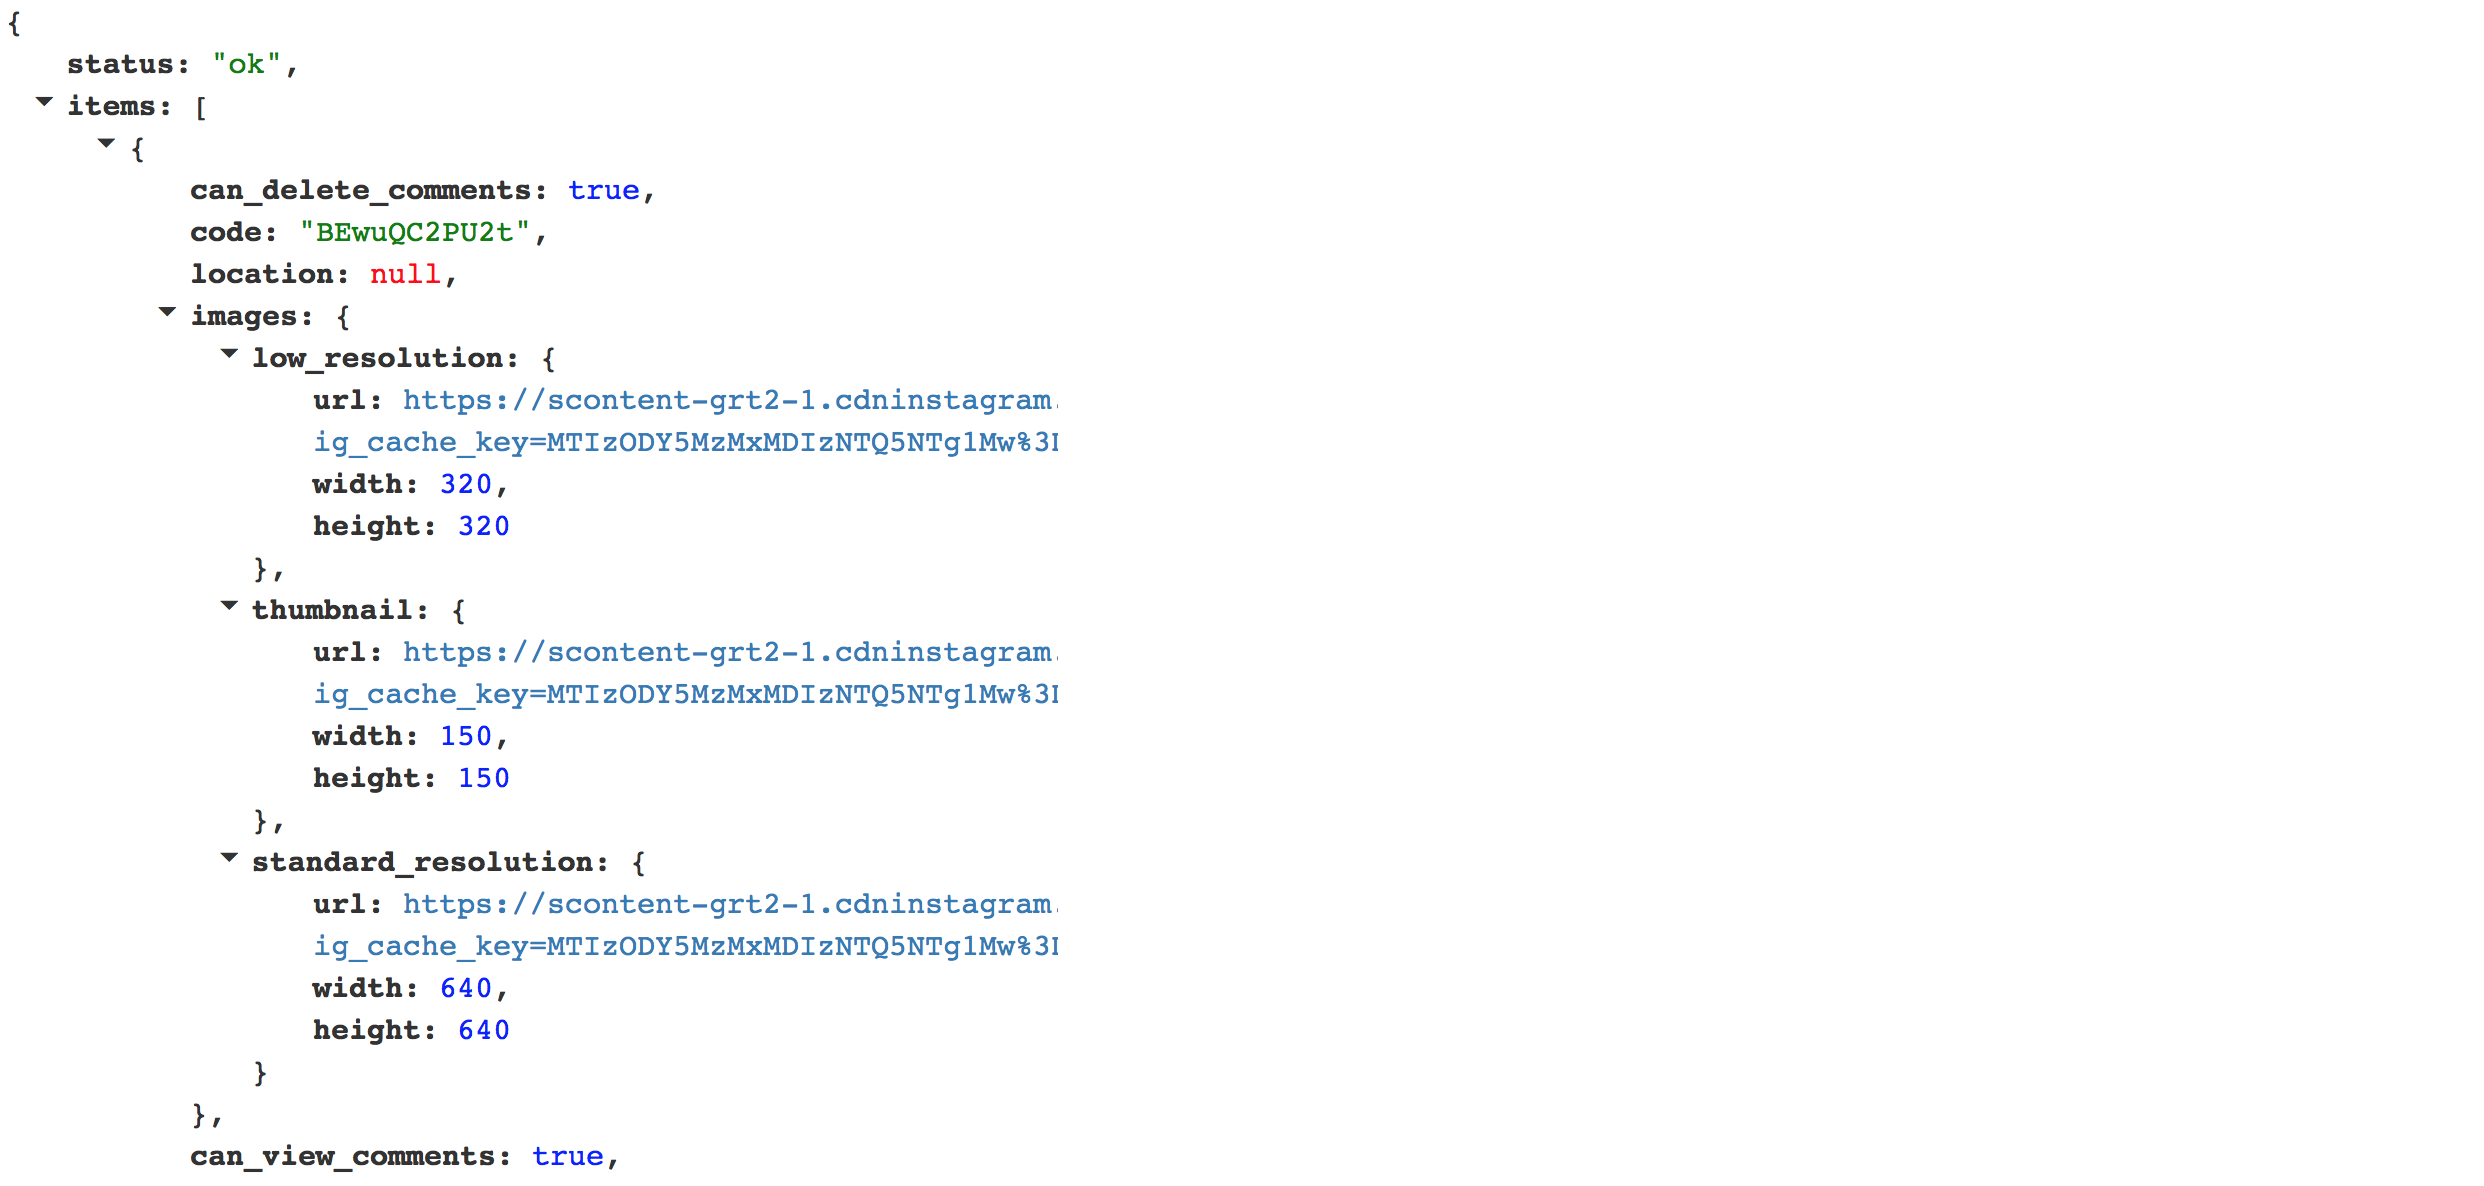
\includegraphics[width=1.5\textwidth]{fig2}
\caption{Exemplo do JSON da API do Instagram}
\end{figure}
	
	A quinta e última etapa é realizar um \textit{wget} para baixar as imagens encontradas e logo após movê-las para suas respectivas pastas.
	
\section{Produto esperado}
	O produto esperado é um parser completo para download fácil das fotos de usuário de qualquer perfil público no Instagram.

\end{document}
